\message{ !name(LaMain.tex)}\documentclass[romanian,12pt,a4paper]{article}

% Set up page geometry
\usepackage[a4paper,margin=2.5cm]{geometry}

% Font setup
\usepackage{fontspec}
\setmainfont{New York Small}

% Line spacing
\usepackage{setspace}
\onehalfspacing


% Other useful packages
\usepackage{amsmath,amssymb,amsthm} % Math packages
\usepackage{graphicx} % For including images
\usepackage[hidelinks]{hyperref} % For hyperlinks in PDF
\usepackage[romanian]{babel} % Language setting
%\usepackage{csquotes} % For quotations
\usepackage[backend=biber,style=vancouver]{biblatex}
\addbibresource{My_Library.bib}

% Document info
\title{Spondilodiscite}
\author{Nicolas}
\date{}

\begin{document}

\message{ !name(LaMain.tex) !offset(-3) }


	\maketitle

\pagebreak
\section{Introducere}

\begin{itemize}
\item
  Introducerea se va redacta spre final latex
\end{itemize}
\pagebreak
\section{Epidemiologie}

Spondilodiscita reprezintă o inflamație infecțioasă a discului
intervertebral și a corpurilor vertebrale adiacente, fiind o afecțiune
rară, dar gravă, cu potențial de a provoca distrugeri structurale
semnificative și complicații neurologice. Etiologia poate fi variată,
incluzând infecții bacteriene piogene, infecții tuberculoase și, mai
rar, fungice. În practica clinică, spondilodiscita este
deosebit de importantă datorită diagnosticului adesea tardiv, care poate
conduce la complicații severe precum instabilitatea coloanei vertebrale,
abcesul epidural sau compresiunea măduvei spinării. În plus, infecția
poate progresa subacut, ceea ce complică și mai mult diagnosticarea
precoce.

Capitolul de epidemiologie își propune să ofere o perspectivă detaliată
asupra prevalenței și incidenței spondilodiscitei, identificând totodată
factorii de risc asociați și distribuția geografică a bolii. În acest
context, vor fi prezentate date epidemiologice actuale care evidențiază
diferențele regionale, influența condițiilor socio-economice și evoluția
incidenței în ultimele decenii. Scopul este de a sublinia relevanța
spondilodiscitei în diferite populații și de a evidenția necesitatea
unor strategii eficiente de diagnostic și tratament, având în vedere
tendințele epidemiologice emergente.

\subsection{Prevalență și incidență}

Prevalența spondilodiscitei variază semnificativ la nivel global, fiind
influențată de factori precum accesul la servicii medicale, prevalența
bolilor cronice (de exemplu, diabetul și bolile autoimune), și starea
socio-economică. În țările dezvoltate, prevalența raportată a
spondilodiscitei este de aproximativ 0,4 - 2,4 cazuri la 100.000 de
persoane pe an, cu o ușoară creștere observată în ultimele decenii
datorită îmbunătățirii tehnicilor de diagnosticare și creșterii
numărului de pacienți imunocompromiși \cite{RoleNuclearMedicine2012}. În
regiunile în curs de dezvoltare, prevalența poate fi subraportată din
cauza accesului limitat la îngrijirea medicală și a resurselor
diagnostice insuficiente \cite{RadionuclideImagingMusculoskeletal2016}.

Incidența spondilodiscitei variază între 2,2 și 7,4 cazuri la 100.000 de
persoane pe an în țările dezvoltate, cu o incidență mai mare în
populațiile vârstnice și la pacienții cu comorbidități preexistente, cum
ar fi diabetul sau insuficiența renală cronică
\cite{ImagingAssessmentSpine2024}. În țările în curs de dezvoltare,
incidența poate fi mai mare din cauza prevalenței ridicate a
tuberculozei și a altor infecții cronice, dar datele precise sunt adesea
limitate. De exemplu, incidența spondilodiscitei tuberculoase rămâne
semnificativă în anumite regiuni din Asia și Africa, reprezentând o
proporție considerabilă din cazurile globale de spondilodiscită
\cite{RadionuclideImagingMusculoskeletal2016}.

Incidența și prevalența spondilodiscitei au prezentat o creștere
treptată în ultimele decenii, în special în țările dezvoltate. Această
creștere este atribuită în parte îmbunătățirii tehnicilor imagistice,
cum ar fi RMN-ul și PET/CT, care permit o diagnosticare mai precisă și
mai timpurie a afecțiunii. În plus, o proporție mai mare a populației
trăiește mai mult timp cu comorbidități care predispun la
spondilodiscită, cum ar fi diabetul, bolile autoimune și utilizarea pe
termen lung a corticosteroizilor
\cite{RoleNuclearMedicine2012}\cite{ImagingAssessmentSpine2024}.În
același timp, avansul în tratamentele antimicrobiene și în managementul
chirurgical al infecțiilor spinale a contribuit la o scădere a
mortalității și la îmbunătățirea prognosticului pe termen lung pentru
pacienți \cite{RadionuclideImagingMusculoskeletal2016}.

\subsection{Factori de risc}

Vârsta este un factor de risc semnificativ pentru dezvoltarea
spondilodiscitei, incidența crescând odată cu înaintarea în vârstă.
Majoritatea cazurilor sunt raportate la pacienți cu vârste de peste 50
de ani, cu un vârf în jurul vârstei de 70 de ani. În ceea ce privește
sexul, bărbații sunt mai predispuși la spondilodiscită, cu o rată de
incidență mai mare comparativ cu femeile. Această diferență este
atribuită în parte prevalenței mai mari a factorilor de risc, cum ar fi
diabetul și consumul de alcool, în rândul bărbaților
\cite{RoleNuclearMedicine2012}.Etnia poate juca, de asemenea, un rol,
deși datele sunt limitate. Anumite grupuri etnice din regiunile cu
prevalență ridicată a tuberculozei, cum ar fi Asia de Sud și Africa
subsahariană, prezintă un risc mai mare de spondilodiscită tuberculoasă
\cite{ImagingAssessmentSpine2024}.

Comorbiditățile joacă un rol central în dezvoltarea spondilodiscitei.
Diabetul zaharat este unul dintre cei mai importanți factori de risc,
pacienții diabetici având un risc semnificativ mai mare de a dezvolta
această afecțiune din cauza statusului lor imun compromisul.
Imunodeficiențele, fie ele congenitale, dobândite (de exemplu, HIV/SIDA)
sau iatrogene (de exemplu, tratamente cu corticosteroizi pe termen
lung), cresc de asemenea riscul de spondilodiscită. Utilizarea de
droguri intravenoase este un alt factor de risc major, legat de
introducerea directă a patogenilor în circulația sanguină, ceea ce poate
duce la infecții hematogene ale coloanei vertebrale
\cite{RadionuclideImagingMusculoskeletal2016}\cite{ImagingAssessmentSpine2024}.

Condițiile socio-economice precare sunt strâns legate de o incidență mai
mare a spondilodiscitei. Accesul limitat la servicii medicale și
diagnostic precoce, igiena precară, nutriția deficitară, și ratele mai
mari de infecții cronice, cum ar fi tuberculoza, contribuie la riscul
crescut de spondilodiscită în populațiile defavorizate. În țările în
curs de dezvoltare, unde accesul la îngrijire medicală este limitat și
prevalența tuberculozei este ridicată, spondilodiscita tuberculoasă este
mai frecventă. În contrast, în țările dezvoltate, riscul este mai mare
la pacienții vârstnici și imunocompromiși din cauza incidenței crescute
a bolilor cronice și a utilizării pe termen lung a terapiilor
imunosupresive \cite{RoleNuclearMedicine2012}.

\subsubsection{Grupe populaționale vulnerabile}

Analiza epidemiologică a spondilodiscitei în populația pediatrică și
geriatrică arată o creștere semnificativă a incidenței în rândul
vârstnicilor, în special în Germania, unde 59.6\% dintre cazuri apar la
pacienți cu vârsta de 70 de ani și peste. Staphylococcul și Escherichia
coli sunt principalii agenți patogeni implicați. În contrast, la copii,
studiile din Coreea de Sud indică faptul că S. aureus și M. tuberculosis
sunt cauzele predominante ale spondilodiscitei, ceea ce subliniază
diferențele importante în etiologie între cele două grupe de vârstă
\cite{EtiologyClinicalPresentation2016}

Prevalența spondilodiscitei este semnificativ mai mare în rândul
pacienților imunocompromiși, în special în cei cu HIV/SIDA, cancer, sau
cei supuși transplanturilor. Acești pacienți sunt expuși unui risc
crescut de a dezvolta infecții severe, inclusiv spondilodiscită,
datorită stării lor imunitare compromise. În Iran, seroprevalența
toxoplasmozei a fost de 45.9\% în rândul pacienților cu HIV/SIDA și
43.6\% în pacienții cu cancer, subliniind vulnerabilitatea acestor grupe
la infecții opportunistice \cite{EpidemiologySpondylodiscitisGermany2023}
\pagebreak
\section{Rolul imagisticii în diagnostic și tratament}

\subsection{Ghidarea procedurilor de biopsie}

Un stiudiu a evidențiat că biopsia percutanată ghidată imagistic
reprezintă o metodă sigură și eficientă pentru confirmarea
diagnosticului de spondilodiscită și pentru identificarea
microorganismului implicat. Printre modalitățile imagistice disponibile,
tomografia computerizată (CT) este de departe cea mai utilizată și
eficientă pentru ghidarea acestei proceduri, datorită capacității sale
de a asigura accesul sigur la structurile spinale, inclusiv la leziuni
mici. CT-ul depășește în precizie ghidarea fluoroscopică, fiind capabil
să ghideze intervențiile în toate regiunile scheletice, inclusiv
segmentele coloanei vertebrale \cite{PercutaneousCTGuidedBone2023}.

Un alt studiu efectuat de Chang et al. a evidențiat că randamentul
diagnostic microbiologic nu este influențat în mod semnificativ de
metoda de ghidare imagistică utilizată, CT sau angiografie. Cu toate
acestea, locul de prelevare a probelor de biopsie joacă un rol crucial
în obținerea unui diagnostic precis. Astfel, biopsiile efectuate din
discurile intervertebrale sau țesuturile moi paravertebrale au prezentat
un randament diagnostic de 64,8\%, comparativ cu 45,5\% în cazul
biopsiilor din platourile osoase (p \textless{} 0,001). Studiul a
indicat că biopsiile din discurile intervertebrale și țesuturile moi
paravertebrale sunt mai eficiente decât cele din os și platourile
vertebrale în obținerea unui randament diagnostic microbiologic optim.
De asemenea, administrarea de antibiotice înainte de procedură nu
influențează în mod semnificativ rezultatele biopsiei
\cite{ImageGuidedBiopsyAcute2023}. În figura
\phantomsection\label{biop-48}{} este o biopsie ghidată angiografic.

Utilizarea ghidării cu ultrasunete în procedurile spinale este limitată,
fiind indicată în principal în cazuri particulare, cum ar fi prezența
unui abces paravertebral voluminos
\cite{UltrasoundGuidedPercutaneousBone2023}.

\begin{figure}
\centering
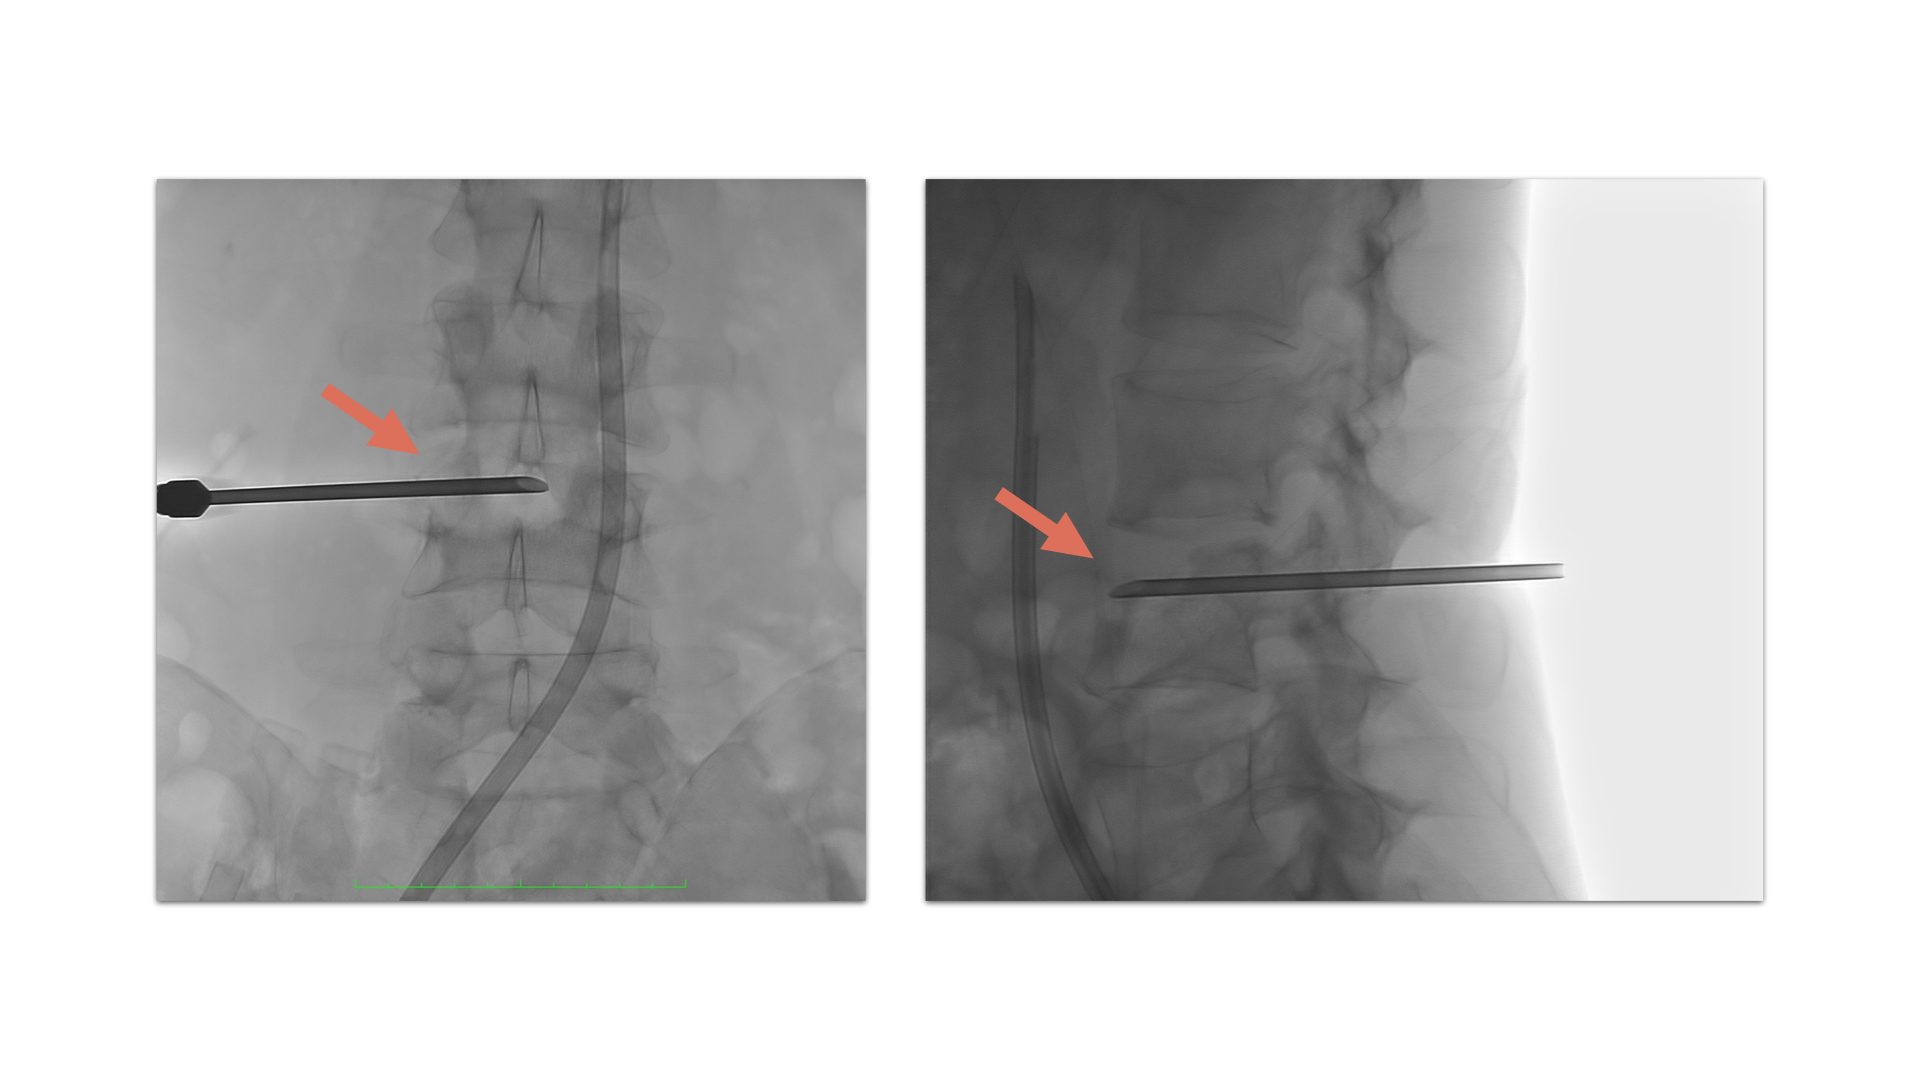
\includegraphics[width=\textwidth]{Files/biop-48.png}
\caption{Biopsie ghidată angiografic la un pacient de 48 de ani,
prezentat cu dorsalgii lombare intense, febră și frisoane, efectuată la
nivelul vertebrei L4 (vedere axială în stânga---reconstrucție sagitală
în dreapta) confirmă diagnosticul de spondilodiscită. Acul de biopsie (8
gauge) este poziționat în corpul vertebral L4, evidențiindu-se eroziunea
plăcii terminale superioare (săgeți) adiacentă discului}
\end{figure}

\phantomsection\label{biop-48}{}

\subsection{Monitorizarea răspunsului la tratament}

Pentru monitorizarea eficacității tratamentului în spondilodiscită,
markerii imagistici utilizati includ reducerea edemului tisular,
stabilizarea sau îmbunătățirea integrității osoase și a structurilor
discale, precum și dispariția sau diminuarea abceselor paravertebrale.
În particular, imagistica prin rezonanță magnetică (IRM) este preferată
pentru urmărirea atât a pacienților tratați conservator, cât și a celor
operați. IRM poate arăta modificări în inflamația țesuturilor moi,
scăderea semnelor de infecție ososă și, uneori, chiar regresia completă
a acestor semne, cum ar fi reducerea semnificativă a gadolinofiliei la
nivelul țesutului osos sau în spațiul epidural.
\cite{CorrelationFollowupMRI2020}\cite{SpondylodiscitisUpdateDiagnosis2010}

În ceea ce privește intervalele de urmărire, reevaluarea imagistică se
recomandă la 4-6 săptămâni de la inițierea tratamentului, mai ales
pentru a evalua răspunsul la terapia antimicrobiană și pentru a ajusta
tratamentul dacă este necesar. În cazurile de spondilodiscită cronică
sau complicată, reevaluările ulterioare pot fi necesare la 3 luni și
ulterior, în funcție de evoluția clinică și imagistică. Este important
de menționat că, în unele cazuri, modificările imagistice pot persista
chiar și după ameliorarea clinică, ceea ce subliniază necesitatea unei
evaluări riguroase care să includă atât criterii clinice, cât și
radiologice
\cite{CorrelationFollowupMRI2020}\cite{ImagingAssessmentSpine2024}

\subsection{Planificarea chirurgicală}

\subsubsection{Indicații chirurgicale}

Imagistica preoperatorie este esențială în identificarea corectă a
indicațiilor pentru intervenția chirurgicală la pacienții cu
spondilodiscită. Tratamentul chirurgical este indicat atunci când IRM
arată compresie a rădăcinilor nervoase, a măduvei spinării sau a durei
mater, cum ar fi în cazul unui abces epidural cu proeminență a
ligamentului longitudinal anterior. Instabilitatea coloanei vertebrale
din cauza distrugerii osoase sau deformităților severe, cum ar fi
cifoza, sunt, de asemenea, indicații clare pentru intervenție
chirurgicală. Evacuarea chirurgicală a unui abces anterior este necesară
atunci când acesta depășește 2,5 cm și, în cazul distrugerii
concomitente a corpului vertebral, trebuie efectuat debridementul osos
urmat de reconstrucție. Tratamentul medical nereușit, inclusiv biopsiile
negative sau durerea persistentă, poate indica necesitatea intervenției
chirurgicale, cu condiția să existe o cauză obiectivă potențială. În
multe cazuri de spondilodiscită tuberculoasă, abcesul și osul sequestrat
și discul sunt atât de extinse încât chirurgii preferă o abordare
chirurgicală combinată cu chimioterapie. Interesant este că mulți
pacienți răspund mai bine la tratament chirurgical atunci când boala
este activă decât atunci când tuberculoza este deja vindecată
\cite{SurgicalTreatmentSpondylodiscitis2012}

\subsubsection{Evaluarea imagistică postoperatorie}

Evaluarea imagistică postoperatorie joacă un rol crucial în
monitorizarea succesului intervenției chirurgicale și în detectarea
precoce a complicațiilor. IRM este utilizată frecvent pentru a verifica
reducerea inflamației, rezolvarea abceselor și stabilizarea structurilor
vertebrale. De asemenea, CT-ul este util pentru evaluarea poziționării
implanturilor și stabilității mecanice a coloanei vertebrale.
Reevaluările imagistice la intervale regulate, cum ar fi la 4 și 6
săptămâni postoperator, sunt recomandate pentru a asigura o recuperare
adecvată și pentru a ajusta planul de tratament în funcție de evoluția
clinică și imagistică \cite{RetrospectiveStudySpondylodiscitis2020}
\pagebreak
\section{Tehnici de imagistică}

În diagnosticul spondilodiscitei (SD), diverse modalități imagistice
oferă perspective diferite asupra manifestărilor și stadiilor bolii.
Radiografia convențională, deși adesea prima metodă utilizată datorită
accesibilității și rapidității sale, are sensibilitate și specificitate
limitate în stadiile inițiale ale infecției. Cu toate acestea, poate
identifica modificări osoase semnificative în etapele avansate.
Tomografia computerizată (CT) aduce o valoare adăugată când imagistica
prin rezonanță magnetică (IRM) este contraindicată, oferind o evaluare
detaliată a distrucțiilor osoase și a extinderii infecției la
structurile adiacente. În contrast, IRM-ul se impune ca standardul de
aur în evaluarea spondilodiscitei, datorită capacității sale superioare
de a diferenția între diversele stadii ale bolii și de a caracteriza mai
precis țesuturile moi și structurile osoase. Această secțiune va explora
avantajele și limitările fiecărei modalități imagistice, subliniind
importanța integrării lor în stabilirea unui diagnostic corect și în
managementul adecvat al spondilodiscitei.

\subsection{Radiologia convențională}

Radiografia convențională are o sensibilitate și specificitate redusă
(82\% și 57\%, respectiv) pentru diagnosticul spondilodiscitei (SD) dar,
este adesea prima metodă utilizată pentru evaluarea durerilor de spate.
Radiografia convențională poate evidenția diverse manifestări ale
spondilodiscitei în funcție de stadiul bolii. În stadiile precoce,
eroziunea subcondrală este considerată primul semn identificabil prin
această metodă. La 3-6 săptămâni de la infecție, pot apărea fragmentarea
sau eroziunea unghiului anterior al plăcii vertebrale, reducerea
spațiului intervertebral, pierderea lordozei fiziologice și deformarea
structurală. Manifestările târzii, după 8-12 săptămâni, includ scleroza
reactivă și formarea de punți osoase între vertebre. Cu toate acestea, o
radiografie cu aspect normal nu poate exclude o spondilodiscită
\cite{SpondylodiscitisDiagnosisTreatment2017}. În imaginile prezentate de
\emph{Crombé et al.} în \ref{rx-general} sunt
radiografiile de profil a doi pacienți cu spondilodiscită și ilustrează
aspectele imagistice radiografice a patologiei.

\begin{figure}\label{rx-general}
\centering
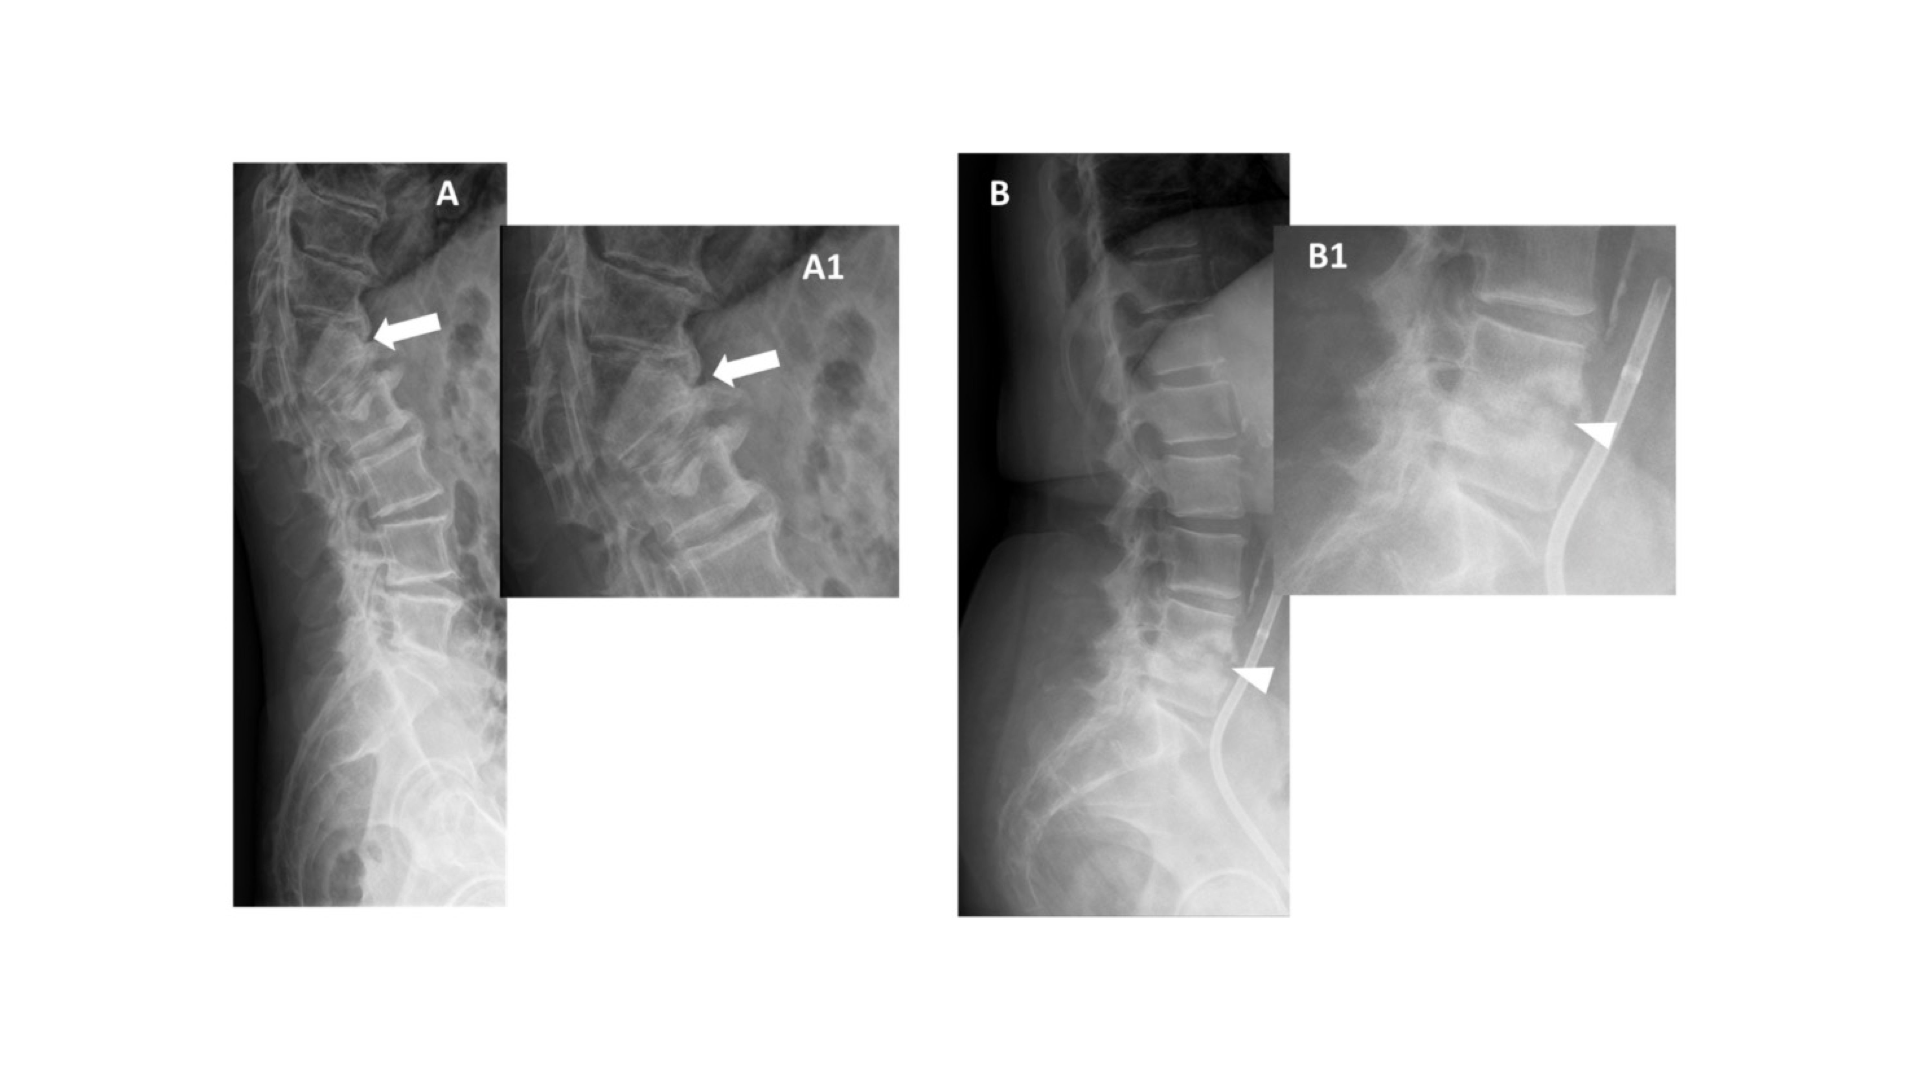
\includegraphics[width=\textwidth]{Files/rx-general.png}
\caption{Radiografiile convenționale în incidență laterală (Panoul A și
detaliul A1) ilustrează cazul unui pacient de 77 de ani cu antecedente de
spondilodiscită piogenă la nivelul corpurilor vertebrale T12-L1,
observându-se colaps parțial și fuziune vertebrală (săgeți). În mod
similar, radiografiile convenționale în incidență laterală (Panoul B și
mărirea B1) prezintă o pacientă de 64 de ani cu spondilodiscită la
nivelul corpurilor vertebrale L4-L5, evidențiindu-se eroziuni pronunțate
ale platourilor vertebrale (capetele de săgeți)
\cite{ImagingSpondylodiscitisComprehensive2024}.}
\end{figure}


\subsubsection{Sensibilitate și specificitate}

Radiografiile simple au o sensibilitate și specificitate redusă în
diagnosticul spondilodiscitelor, în special în stadiile incipiente ale
infecției
\cite{SuggestionsManagingPyogenic2007}\cite{SpinalInfections2005}\cite{ImagingSpondylodiscitisComprehensive2024}.
În tuberculoza spinală, de exemplu, radiografiile arată o sensibilitate
de 82\% și o specificitate de 57\% \cite{SpinalInfectionsClinical2014},
indicând un risc semnificativ de rezultate fals negative sau fals
pozitive.

\subsubsection{Acuratețea diagnostică}

Această metodă diagnostică necesită o reducere de 30\% până la 40\% a
matricei osoase pentru a evidenția pierderea osoasă, ceea ce poate
întârzia identificarea precoce a patologiei. Pot detecta semne evidente
ale bolii după 8-12 săptămâni, precum eroziunea platourilor vertebrale
și reducerea spațiului intervertebral, dar sunt limitate în
identificarea modificărilor subtile. Limitările lor în detectarea
precoce și în diferențierea precisă a patologiilor infecțioase de cele
degenerative pot necesita utilizarea unor investigații suplimentare mai
costisitoare pentru confirmarea diagnosticului
\cite{SpinalInfectionsClinical2014}.

\subsubsection{Disponibilitate și considerente de cost}

Radiografiile simple sunt larg accesibile și relativ ieftine în
comparație cu alte metode imagistice avansate, cum ar fi RMN-ul sau
CT-ul. Acestea sunt disponibile în majoritatea instituțiilor medicale,
inclusiv în zonele cu resurse limitate, ceea ce le face o opțiune
practică pentru evaluarea inițială a pacienților. Costul redus și
accesibilitatea ridicată le permit să fie utilizate pe scară largă,
inclusiv pentru monitorizarea pe termen lung a pacienților
\cite{ImagingSpondylodiscitisComprehensive2024}.

\subsection{Tomografia computerizată}

Tomografia computerizată (CT) reprezintă o modalitate imagistică
alternativă valoroasă în contextul contraindicațiilor pentru imagistica
prin rezonanță magnetică (IRM), cum ar fi prezența dispozitivelor
cardiace incompatibile cu IRM sau a altor factori specifici pacientului.
Deși contribuția sa în procesul diagnostic general este relativ
limitată, CT-ul excelează în anumite domenii specifice. Acesta
facilitează identificarea, caracterizarea și cuantificarea extinderii
proceselor osteolitice, vizualizarea modificărilor patologice ale
țesuturilor paravertebrale și îngroșarea țesutului adipos adiacent. Mai
mult, CT-ul cu substanță de contrast îmbunătățește semnificativ
acuratețea diagnosticului abceselor și optimizează ghidajul procedurilor
intervenționale, cum ar fi biopsia cu ac fin sau drenajul abceselor. În
pofida acestor avantaje, rolul primordial al CT-ului în patologia
spinală rămâne preponderent în sfera planificării preoperatorii a
intervențiilor chirurgicale, unde oferă informații anatomice, esențiale
pentru o abordare chirurgicală optimă
\cite{DiagnosticInterventionalManagement2020}.

\subsubsection{Sensibilitate și specificitate}

Tomografia computerizată (CT) prezintă o sensibilitate și specificitate
variabilă în evaluarea spondilodiscitei, în funcție de tipul de infecție
și stadiul bolii. Un studiu a raportat o sensibilitate generală de 79\%
pentru detectarea infecțiilor spinale, inclusiv abcesul epidural spinal
(SEA), osteomielita vertebrală și alte infecții paravertebrale
\cite{ImagingCharacteristicsCT2022}. Totuși, sensibilitatea pentru
detectarea SEA a fost semnificativ mai scăzută, de doar 18\%
\cite{ImagingCharacteristicsCT2022}. Alte studii au raportat
sensibilități de până la 90\% pentru diverse patologii infecțioase ale
coloanei vertebrale, evidențiind variabilitatea în funcție de tehnică și
expertiza radiologului \cite{ImagingAssessmentSpine2024}.

CT-ul poate detecta modificări osoase și ale țesuturilor moi mai devreme
decât radiografiile, dar are o sensibilitate și specificitate mai
scăzute pentru detectarea abceselor epidurale comparativ cu alte tipuri
de infecții. Aceste valori pot varia considerabil în funcție de
specificul patologiei evaluate și de interpretarea radiologică
\cite{ImagingCharacteristicsCT2022}\cite{ImagingAssessmentSpine2024}.

\subsubsection{Acuratețea diagnostică}

CT-ul este util în diagnosticarea precoce a modificărilor structurale
ale oaselor și a formării abceselor. în imaginile preluate din articolul
publicat de \emph{Crombé et al.} în \phantomsection\ref{CT-general}{}
sunt reprezentate imaginile CT a unui pacient de 77 de ani diagnosticat
cu SD piogenă. În ciuda sensibilității sale limitate în detectarea unor
afecțiuni precum SEA, este valoroasă pentru vizualizarea detaliată a
leziunilor și a extinderii acestora, contribuind astfel la o evaluare
comprehensivă a pacienților cu suspiciune de infecție spinală
\cite{ImagingCharacteristicsCT2022}\cite{ImagingAssessmentSpine2024}.

\begin{figure}
\centering
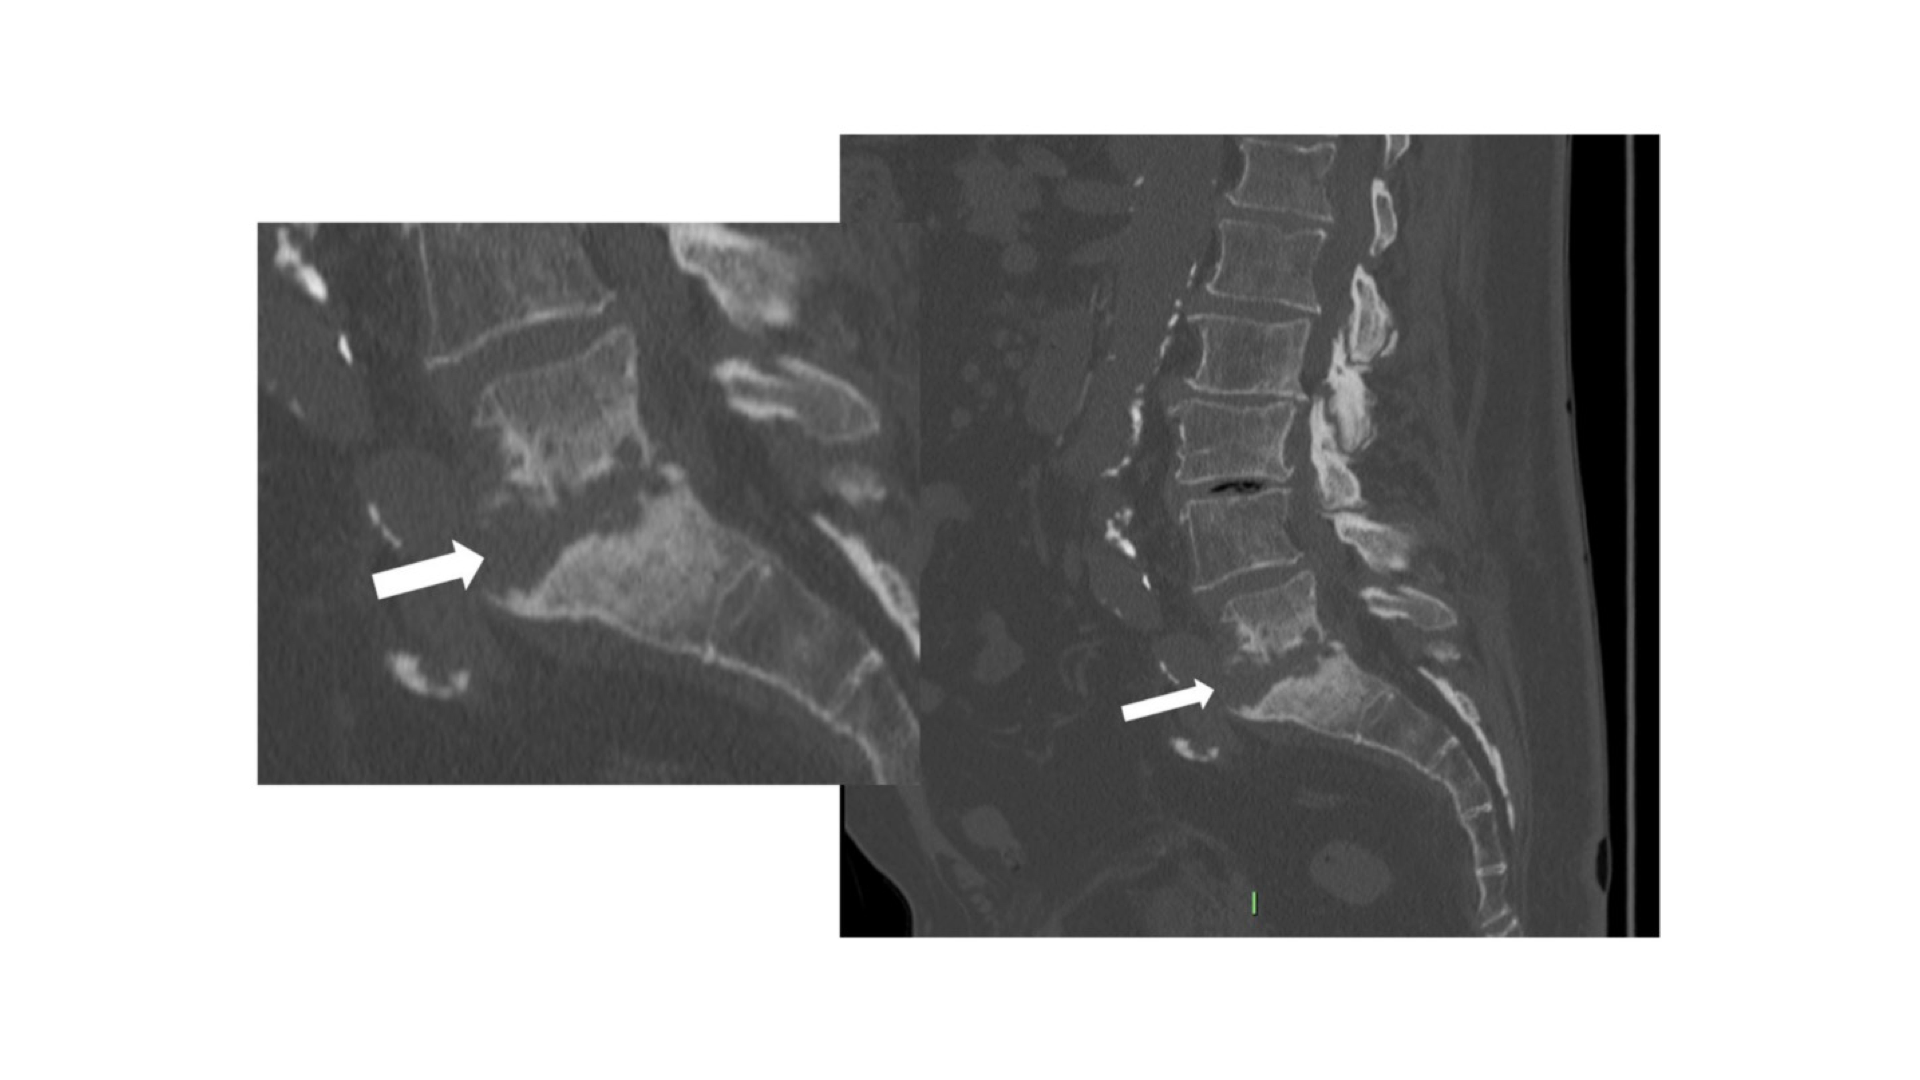
\includegraphics[width=\textwidth]{Files/CT-general.png}
\caption{Reconstrucția sagitală CT (în stânga este o imagine mărită)
prezintă o pacientă de 77 de ani diagnosticată cu spondilodiscită
piogenă la nivelul L5-S1, caracterizată prin eroziuni pronunțate ale
platourilor vertebrale (săgeți)
\cite{ImagingSpondylodiscitisComprehensive2024}.}
\end{figure}

\phantomsection\label{CT-general}{}

\subsubsection{Disponibilitate și considerente de cost}

CT-ul este o metodă de imagistică disponibilă pe scară largă și este mai
accesibilă decât imagistica prin rezonanță magnetică (IRM), atât în
termeni de costuri cât și de disponibilitate în unitățile medicale.
Aceasta face ca CT-ul să fie adesea preferat ca primă linie de evaluare
în situațiile de urgență sau în cazurile în care IRM-ul nu este
disponibil \cite{ImagingCharacteristicsCT2022}. De asemenea, poate fi
utilizat pentru ghidarea biopsiilor în scop diagnostic, oferind astfel o
metodă non-invazivă de obținere a materialului pentru analize
microbiologice
\cite{ImagingCharacteristicsCT2022}\cite{ImagingAssessmentSpine2024}.

\subsection{Medicina nucleară}

\subsubsection{Sensibilitate și specificitate}

Medicina nucleară joacă un rol important în diagnosticarea
spondilodiscitei, oferind date comparative valoroase privind
sensibilitatea și specificitatea diferitelor modalități imagistice.
Scintigrafia osoasă cu Technetium-99m (Tc-99m) are o sensibilitate de
aproximativ 90\%, dar o specificitate mai redusă, de 78\%, datorită
rezultatelor fals pozitive cauzate de modificările degenerative.
Scintigrafia cu Gallium-67, deși mai specifică, este adesea utilizată
complementar pentru a îmbunătăți specificitatea studiului și pentru a
detecta locurile de infecție extraosoase. Imagistica cu leucocite
marcate, deși nu este foarte utilă în diagnosticul spondilodiscitei,
poate aduce informații valoroase în anumite cazuri clinice
\cite{RadionuclideImagingMusculoskeletal2016}\cite{RoleNuclearMedicine2012}\cite{ImagingAssessmentSpine2024}
.

O meta-analiză privind utilizarea PET/CT cu Fluorodeoxiglucoză
(FDG-PET/CT) în diagnosticul spondilodiscitei a raportat o sensibilitate
combinată de 97\% și o specificitate de 88\%, evidențiind astfel
potențialul ridicat al acestei tehnici pentru identificarea infecțiilor
spinale și evaluarea răspunsului la tratament
\cite{ImagingAssessmentSpine2024}.

\subsubsection{Acuratețea diagnostică}

Medicina nucleară oferă o acuratețe diagnostică ridicată în evaluarea
spondilodiscitei. FDG-PET/CT, în special, a demonstrat o sensibilitate
și specificitate superioară în comparație cu alte tehnici imagistice,
permițând o localizare precisă a infecției și o evaluare detaliată a
răspunsului la tratament. Cu toate acestea, specificitatea redusă a
scintigrafiei osoase limitează utilizarea acesteia ca metodă unică de
diagnostic
\cite{RadionuclideImagingMusculoskeletal2016}\cite{RoleNuclearMedicine2012}
.

\subsubsection{Disponibilitate și considerente de cost}

Tehnicile de medicină nucleară, cum ar fi FDG-PET/CT, pot fi mai
costisitoare și mai puțin disponibile decât metodele imagistice
convenționale, cum ar fi RMN-ul sau CT-ul. Deși oferă avantaje
semnificative în diagnosticul precis al spondilodiscitei, costurile
ridicate și disponibilitatea limitată pot restricționa utilizarea lor
largă în practica clinică \cite{ImagingAssessmentSpine2024}.

\subsection{Imagistica prin rezonanță magnetică}

Imagistica prin rezonanță magnetică (IRM) se distinge ca instrumentul
imagistic primordial în domeniul neuroradiologic, atât pentru
diagnostic, cât și pentru intervenții, datorită contrastului său
excelent în țesuturile moi și capacității multiplanare. În prezent,
IRM-ul este considerat standardul de aur în diagnosticul
spondilodiscitei (SD), demonstrând o sensibilitate și specificitate
ridicate (92\% și, respectiv, 96\%), în special în stadiile incipiente
ale bolii
\cite{SpondylodiscitisDiagnosisTreatment2017}\cite{CurrentDiagnosisTreatment2008}
. Această performanță se datorează caracterizării superioare a
țesuturilor și abilității de a identifica edemul osos și zonele cu
vascularizație anormală. Edemul osos, un indicator precoce al bolii, se
manifestă prin infiltrat inflamator și expansiunea spațiului
extracelular. Creșterea conținutului de apă se traduce prin
hipointensitate în secvențele T1 și hiperintensitate în secvențele T2
\cite{SpinalInfectionState2013}. Unii autori sugerează că
hiperintensitatea T2 a mușchilor psoas poate fi un semn foarte precoce
al SD lombare \cite{ImagingPsoasSign2016}. IRM-ul evidențiază cu
acuratețe și modificările ulterioare sau post-infecțioase, inclusiv
înlocuirea țesutului necrozat cu țesut fibros vascularizat,
transformarea măduvei galbene, fibroza subcondrală și osteoscleroza.
Capacitatea IRM-ului de a diferenția între formele non-piogene (de
exemplu, SD tuberculoasă sau bruceloză) oferă avantaje semnificative în
caracterizarea etiologică a SD, aspect crucial pentru stabilirea unui
tratament adecvat
\cite{SpinalInfectionState2013}\cite{DiagnosticInterventionalManagement2020}.

\begin{figure}
\centering
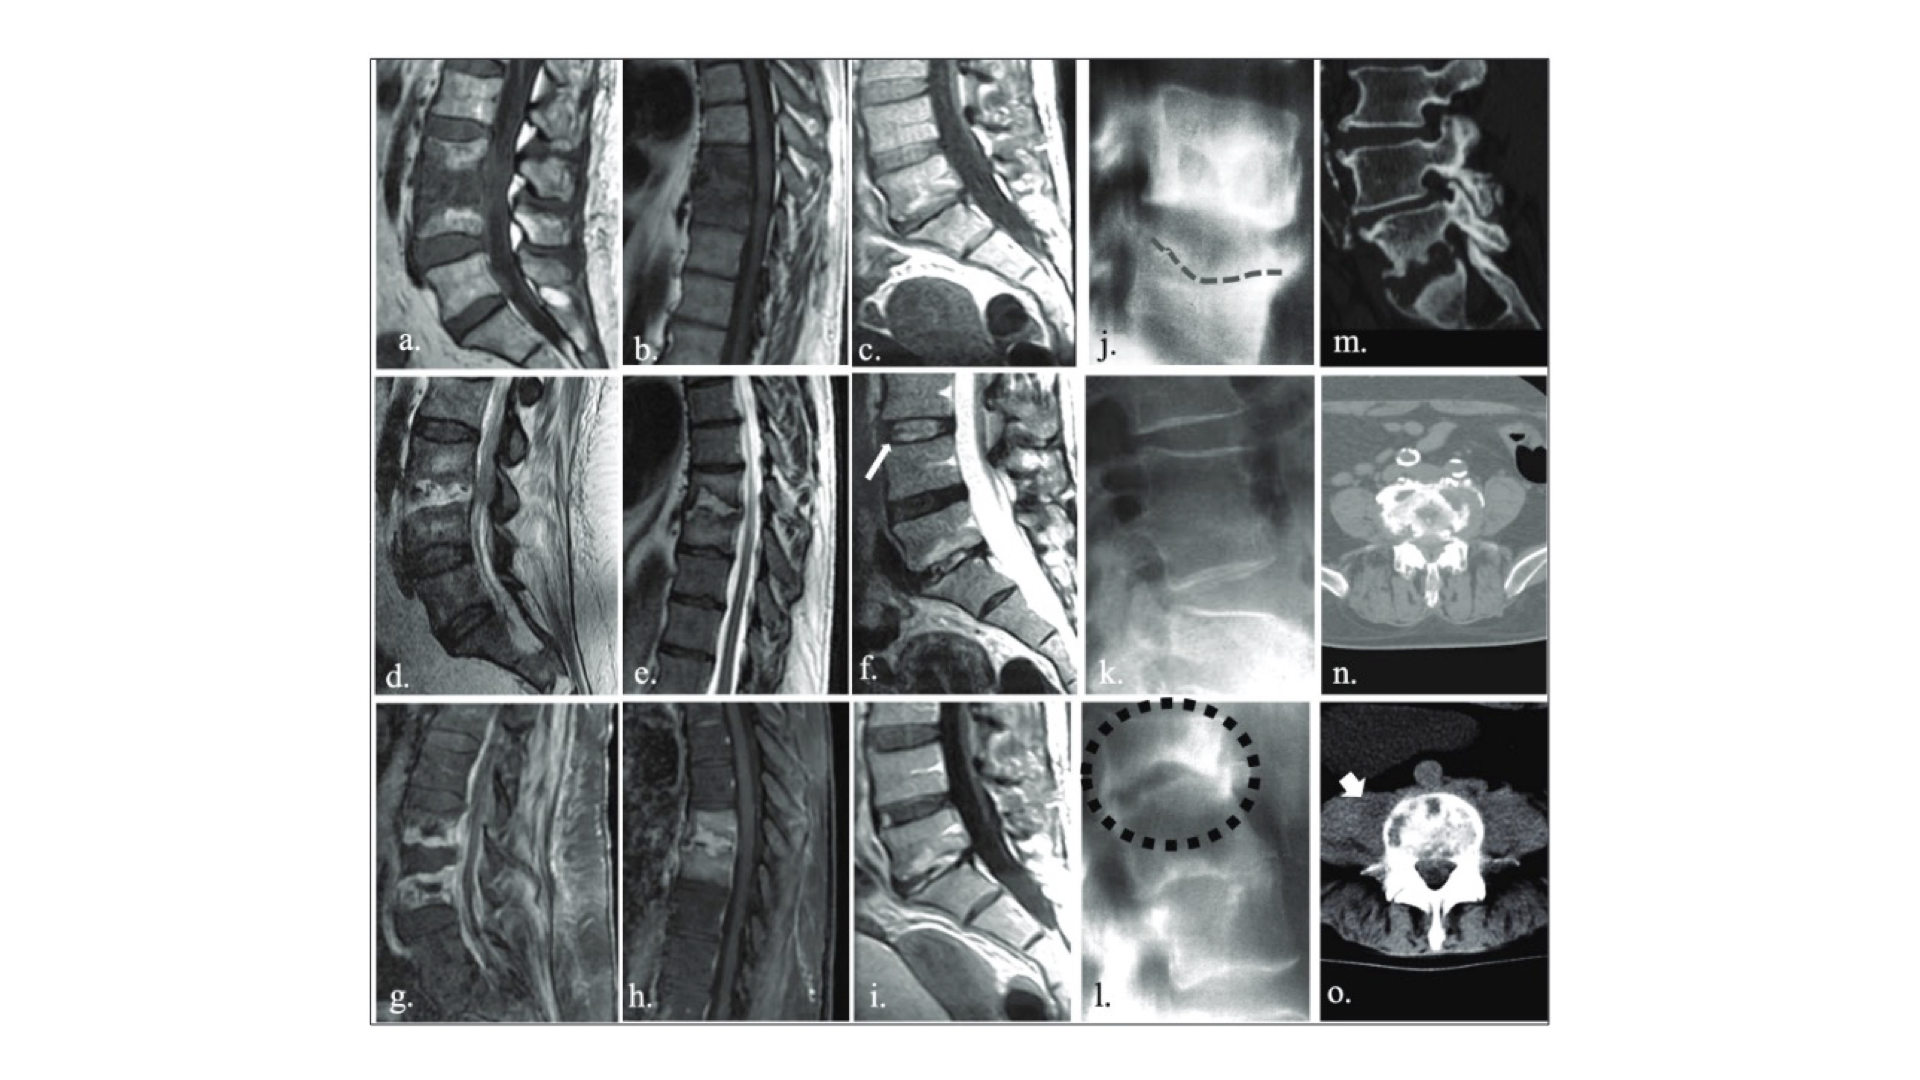
\includegraphics[width=\textwidth]{Files/IRM-important.png}
\caption{Imaginile IRM prezintă o intensitate scăzută a semnalului pe
secvențele T1 (a., b., c.) și o intensitate crescută pe secvențele T2
(d., e., f.), evidențiind modificări atât în discul intervertebral, cât
și în platourile vertebrale. Pierderea fisurii intranucleare normale
(f., săgeata albă) indică alterări ale țesutului fibros din nucleul
pulpos. Vascularizația post-inflamatorie și formarea de țesut
granulomatos pot duce la o intensificare semnificativă a semnalului după
administrarea de contrast (g., h., i.). CR poate detecta eroziunea
subcondrală ca prim semn (j., linia punctată), CT poate evalua osteoliza
și extinderea infecției în țesuturile adiacente (m., n., o., săgeata
albă)
\cite{DiagnosticInterventionalManagement2020}.}\label{IRM-important}
\end{figure}

Imaginea prezentată de \emph{Palumbo et al.} în
\phantomsection\ref{IRM-important}{}, subliniază importanța IRM în
diagnosticarea spondilodiscitei. Conform acestora, imagistica prin
rezonanță magnetică (IRM) este un instrument precis în diagnosticarea
spondilodiscitei, prezentând în mod tipic o intensitate scăzută a
semnalului pe secvențele T1 și o intensitate crescută a semnalului pe
secvențele T2, afectând atât discul intervertebral, cât și platoul
vertebral. Alterările structurale ale discului, cum ar fi pierderea
fisurii intranucleare tipice, indică modificări ale țesutului fibros din
nucleul pulpos. Vascularizația post-inflamatorie și țesutul granulomatos
pot duce la o creștere semnificativă a intensității semnalului după
injectarea cu substanță de contrast (g., h., i.).

În contrast, radiografia convențională (CR) și tomografia computerizată
(CT) sunt mai puțin sensibile, în special în stadiile incipiente ale
infecției. Primul semn observabil pe radiografie este reprezentat de
eroziunea subcondrală (j., linie punctată), vizibilă la 3-6 săptămâni
după infecție. În stadiile ulterioare, se poate observa fuziunea
corpurilor vertebrale (k.) sau colapsul complet al somitelor (l., puncte
negre), în funcție de eficiența tratamentului aplicat. Tomografia
computerizată poate fi utilă în estimarea gradului de osteoliză (m.,
n.), permițând, de asemenea, evaluarea extensiei procesului către
țesuturile perivertebrale (o., săgeata mare)
\cite{DiagnosticInterventionalManagement2020}.

\subsubsection{Sensibilitate și specificitate}

În diagnosticul spondilodiscitei, rezonanța magnetică (RMN) rămâne
metoda preferată datorită sensibilității și specificității sale
ridicate. RMN-ul contrast-enhanced demonstrează o sensibilitate de 97\%,
o specificitate de 93\% și o acuratețe de 94\% în diagnosticarea
spondilodiscitei \cite{ComparisonDiagnosticValue2017}. Aceste valori sunt
semnificativ mai mari comparativ cu alte modalități imagistice,
evidențiind superioritatea RMN-ului în detectarea și caracterizarea
infecțiilor vertebrale.

Secvențele RMN recomandate includ imagistica ponderată T2 cu suprimarea
grăsimii și imagistica ponderată T1 post-contrast cu suprimarea grăsimii
\cite{ComparisonDiagnosticValue2017}. Alternativ, pot fi utilizate
secvențele DIXON T2-WI și T1-WI contrast-enhanced (CE) cu imaginile Fat,
Water, și In-phase. Imagistica ponderată prin difuzie (DWI) este utilă
în cazurile în care pacienții nu pot efectua RMN contrast-enhanced,
oferind informații valoroase despre prezența abceselor și diferențierea
între infecție și modificări degenerative.

\subsubsection{Acuratețea diagnostică}

RMN-ul excelează în dezvăluirea extinderii infecției, oferind imagini
superioare ale țesuturilor moi paraspinale și spațiului epidural.
Spondilodiscita se manifestă prin modificări caracteristice ale
semnalelor RMN, cu intensitate hipo- sau izointensă pe T1 și
hiperintensă pe T2 la nivelul plăcilor subcondrale și discului
intervertebral \cite{DiagnosticPerformanceMultiDetector2022}. Aceste
modificări, împreună cu eroziunile osoase ale plăcilor terminale și
diverse modele de contrast ale plăcii vertebrale, permit o evaluare
detaliată a progresiei bolii.

Modificările degenerative de tip Modic 1 se caracterizează prin platouri
vertebrale hipointense pe secvențele T1 și hiperintense pe T2. În
contrast, spațiul discal apare hipointens atât pe T1, cât și pe T2.
Diferențierea între o infecție și modificările de tip Modic 1 poate fi
dificilă utilizând doar secvențele standard T1 și T2, deoarece semnul
distinctiv major --- creșterea intensității semnalului T2 în discul
intervertebral --- nu este întotdeauna prezent
\cite{DegenerativeDiskDisease1988}.

Adăugarea contrastului poate oferi o claritate superioară, evidențiind
în special componentele epidurale și paraspinale ale infecției prin
priza de contrast distinctă la nivelul discului și al corpurilor
vertebrale. O secvență suplimentară STIR poate furniza informații mai
clare decât T2, datorită saturației grăsimii care accentuează
prelungirea semnalului T2. În situații de urgență sau când există un
volum mare de examinări ale coloanei vertebrale, ar fi mai eficient să
se utilizeze secvențele T1 și STIR, împreună cu câteva secvențe
adiționale, cum ar fi cele cu contrast
\cite{DiffusionweightedMRIClaw2014}.

În ceea ce privește costurile și eficiența, RMN-ul este considerat mai
scump comparativ cu alte tehnici de imagistică, dar beneficiile sale în
diagnosticarea precoce și precisă a spondilodiscitei justifică
investiția. Alternativele, cum ar fi PET/CT cu F-18 FDG, oferă o
sensibilitate de 96\% și specificitate de 95\%, fiind de asemenea
valoroase pentru diagnosticul precoce , dar RMN-ul rămâne standardul de
aur datorită capacității sale de a oferi detalii superioare ale
structurii și extinderii infecției \cite{ComparisonDiagnosticValue2017}.

\subsubsection{Disponibilitate și considerente de cost}

În ceea ce privește disponibilitatea și costurile, RMN-ul este
considerat mai scump comparativ cu alte tehnici de imagistică. Cu toate
acestea, beneficiile sale în diagnosticarea precoce și precisă a
spondilodiscitei justifică investiția. Capacitatea RMN-ului de a oferi
detalii superioare ale structurii și extinderii infecției îl menține ca
standard de aur în evaluarea spondilodiscitei.

Alternativele, cum ar fi PET/CT cu F-18 FDG, oferă o sensibilitate de
96\% și specificitate de 95\%, fiind de asemenea valoroase pentru
diagnosticul precoce \cite{ComparisonDiagnosticValue2017}. Cu toate
acestea, disponibilitatea mai redusă și costurile mai ridicate ale
acestor tehnici avansate pot limita utilizarea lor pe scară largă în
practica clinică curentă.

\subsection{Tehnologii emergente}

Progresele recente în medicina nucleară includ dezvoltarea tehnologiilor
hibride de imagistică, cum ar fi SPECT/CT și PET/MRI. Aceste tehnici
combinate permit obținerea simultană de imagini funcționale și
morfologice, îmbunătățind astfel acuratețea diagnostică și capacitatea
de a evalua extinderea infecției și răspunsul la tratament. De exemplu,
adăugarea componentului CT la scintigrafia osoasă SPECT a crescut
semnificativ sensibilitatea și specificitatea diagnostică, permițând o
localizare mai precisă a infecțiilor
\cite{RadionuclideImagingMusculoskeletal2016}\cite{RoleNuclearMedicine2012}.

\subsection{Tehnici hibride de imagistică}

Utilizarea tehnicilor hibride, cum ar fi PET/CT și SPECT/CT, a
demonstrat îmbunătățiri semnificative în diagnosticul spondilodiscitei.
Aceste metode oferă o evaluare detaliată a metabolismului tisular și a
anatomiei, facilitând diferențierea între infecțiile active și
modificările degenerative. Studiile recente au evidențiat că PET/CT
poate detecta cu mare acuratețe infecțiile spinale, inclusiv în stadiile
incipiente ale bolii
\cite{RadionuclideImagingMusculoskeletal2016}\cite{ImagingAssessmentSpine2024}.
\pagebreak
\section{Methods}
text
\begin{table}
	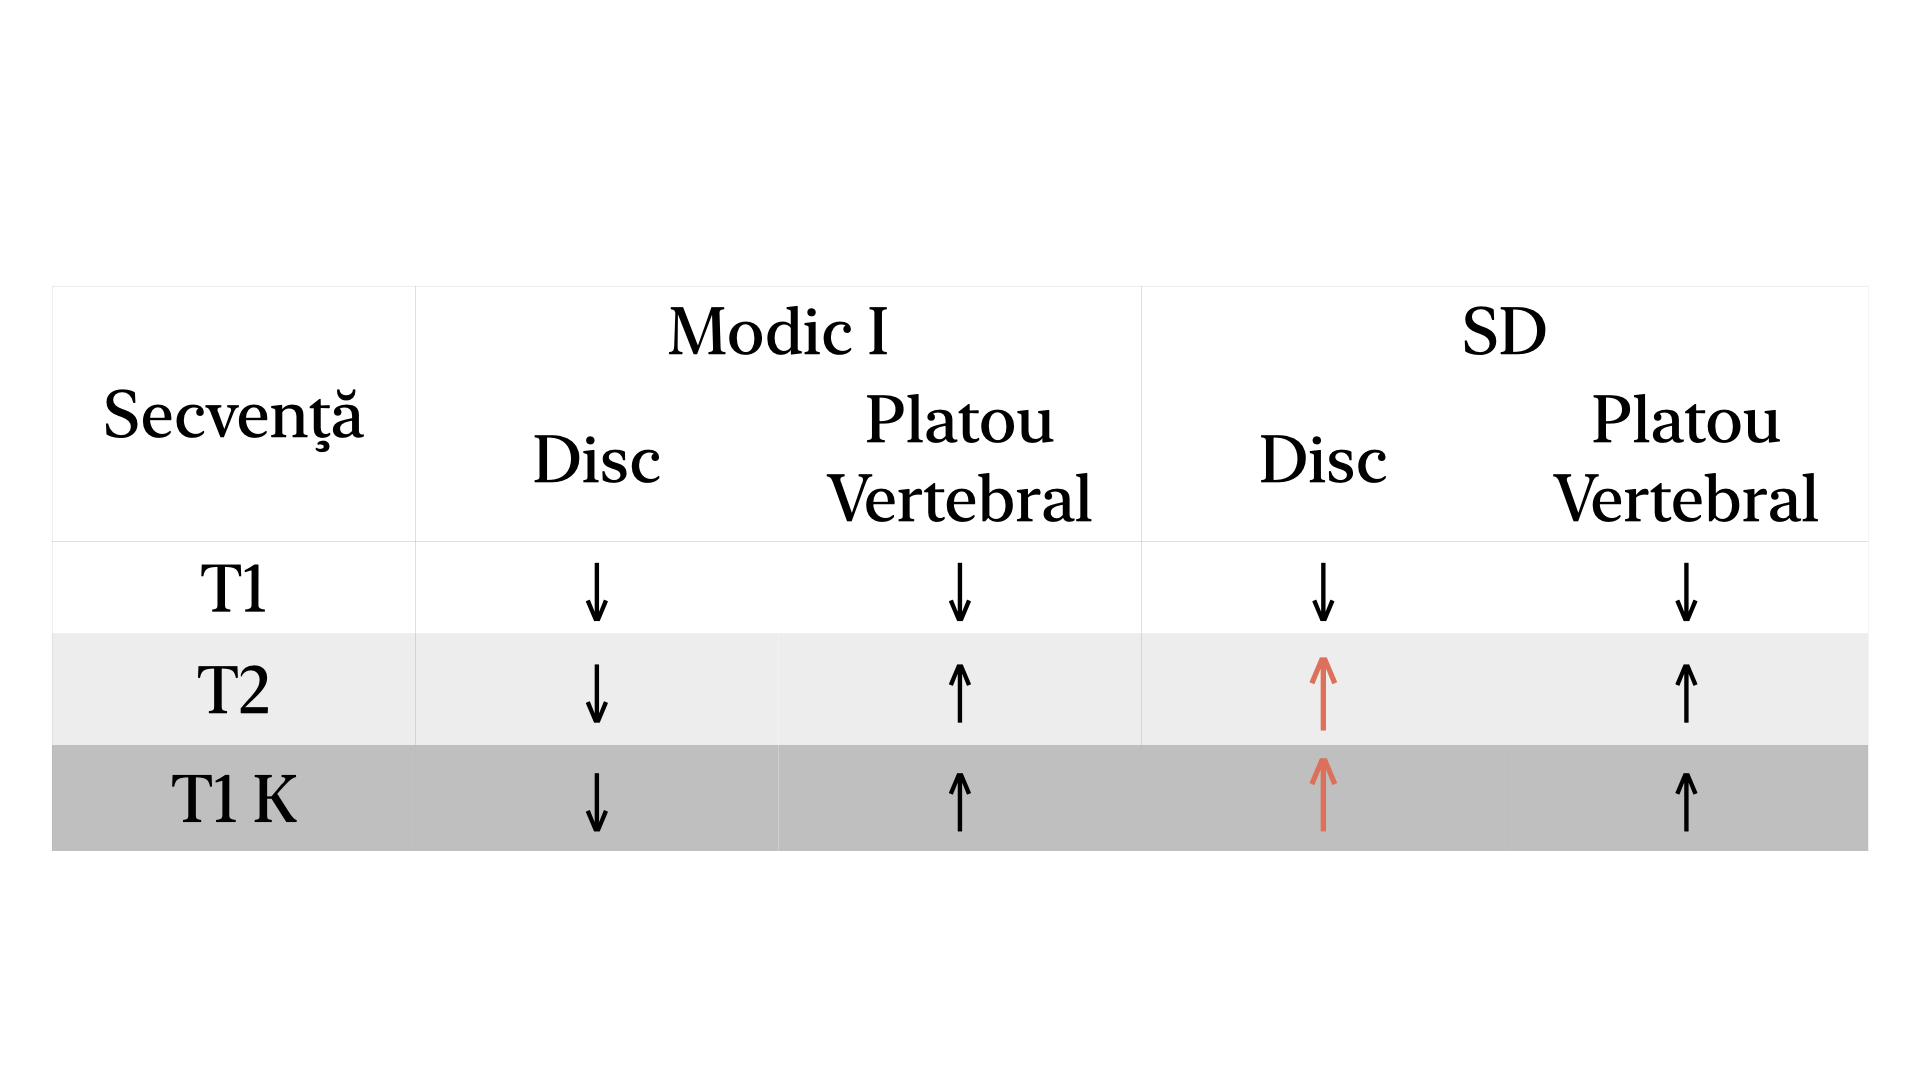
\includegraphics[width=\textwidth]{Files/tb-DSI_vs_MODIC.png}

\end{table}

\pagebreak
\section{Interpretarea datelor}
\pagebreak
\printbibliography[title={Bibliografie}]
\end{document}

\message{ !name(LaMain.tex) !offset(-678) }
